\newpage
\section{Architecture design and technical decisions}
% ------------------------------------------------------------------------------------------------
\subsection{User facing language requirements}
The field of dynamic programming has been influenced in the recent years by a methodology known as Algebraic Dynamic Programming which uses a grammar and an algebra to separate between the parsing and the score computation:
\quote{The Algebraic Dynamic Programming approach (ADP) introduces a conceptual splitting of a DP algorithm into a recognition and an evaluation phase. The evaluation phase is specified by an evaluation algebra, the recognition phase by a yield grammar. Each grammar can be combined with a variety of algebras to solve different but related problems, for which heretofore DP recurrences had to be developed independently. Grammar and algebra together describe a DP algorithm on a high level of abstraction, supporting the development of ideas and the comparison of algorithms.}

Given such formalization \cite{adp} of dynamic programming on sequences, it seems natural to borrow from it and extend it to other types of DP problems. In short, this framework allow the user to define a grammar using parsers, which are then run over an input string and produce intermediate results that are memoized into a table, when multiple solutions are possible, the user can define an aggregation function ($h$) to retain only some candidates for further combination.

The benefits of ADP framework is that it does not constraint the result of the evaluation to be a single value, but can extend parsers to backtracking parsers or pretty-printers. Additionally, we want to support the following features:\ol
%\item {\color{red}\textbf{Cyclic problems:} are inherently very similar to string problems, except that the input is cyclic. To support such problem efficiently, we only need to mark the grammar cyclic such that it would apply on any unfolding of the cyclic input string.}
\item \textbf{Input pair algebra:} the original ADP framework only support single input, we want to support a pair of inputs such that we can treat problem such as Smith Waterman or Needleman-Wunsch. However, it does not make sense to treat more than two sequences because of the $\Omega(n^3)$ storage requirements that limits the problems size more dramatically.
\item \textbf{Windowing}: this can be easily encoded by passing the windowing parameter that limits the computation, then it could be possible to collect either the best or $k$-best results.
\item \textbf{Input restrictions:} since CUDA (and FPGA) cannot operate on an arbitrary Scala classes, we need to restrict the language to primary types (int, float, ... and structures of them). However, we want to preserve the expressiveness available for Scala and impose restrictions on the input and answers available to CUDA. A typical restriction we want to make is that processed structures are of fixed size so that we avoid memory management issues and thread divergence.
\item \textbf{Single-result on devices:} The general ADP framework supports multiple solutions for intermediate results. Such functionality is easy to support in Scala; however, memory management hampers the performance of the GPU implementation. To overcome this issue, the user could manually manage the memory, but this would defeat most of the benefits of automatic code generation. Hence the trade-off solution we propose is to restrict ADP to only one optimal result on CUDA, while leaving the freedom to obtain co-optimal (or even all possible solutions) with the Scala version.

\item \textbf{Automatic backtracking:} Since efficient code has to be devised we imposed restrictions on the output that could be generated by the parsers on devices. However, on the other side, the backtracking information would be of primary interest for the DSL user, hence we would like to to automate the backtracking to fulfill goals of usefulness, efficiency and ease-of-use in device-specific implementation:\ul
	\item Leaving the backtrack implementation to the user would force him to memoize the backtracking information together with the results (backtrack would  grow towards final result and duplicate unnecessarily information), hence requiring both $O(n^3)$ space and memory management features on devices. 
	\item Enforcing automatic backtracking presents the advantage to ensure constant size for intermediate results, hence ensuring an $O(n^2)$ storage requirement. Collecting the backtracking list can be easily done in $O(n)$ and then inverted whether we prefer bottom-up or top-down construction (the backtrack is usually a lattice of nodes that constitute a tree whose leaves are input elements).
	\ule
\item \textbf{Yield analysis:} in the vanilla ADP, the user has to define for each concatenation the minimal and maximal length of the subsequence on each side. Although non-emptiness information is necessary to avoid infinite recursion in the parsers, forcing an explicit definition can become cumbersome for the DSL user. We want to provide an automatic computation of concatenation boundaries, while at the same time leaving the possibility to manually specify it for maximum flexibility.
\ole

The support of these features has the following implications:\ul
\item \textbf{Dependency analysis:} Since we target GPUs (and FPGAs) which are massively parallel architecture, a top-down execution using hash tables is impractical (fallback computation if element is not present is hard to parallelize), hence we need to construct the result tree bottom-up, therefore ensure that the (partial) evaluation order between rules is respected.
\item \textbf{Normalization:} in order to automate the backtracking, we need the rule to present a certain shape so that we can define uniquely the backtracking information (in particular we want to distinguish between alternatives). Also we need to maintain coherency between the Scala and the CUDA version so that they can inter-operate: we would like to reuse the backtracking information (from CUDA) to do actual processing in Scala (for instance pretty-printing or effectively multiplying matrices).

\item \textbf{Optimizations:} An possible optimization is to break down complex rules into simpler ones if they are expressible so; hereby reducing the complexity of the overall algorithm, would the user production grammar not be optimal. Unfortunately this analysis is very involved: we need to solve the following problem:

Given $f$ , find a pair of functions $(f_1,f_2)$ or $(f_3,f_4)$ such that\footnote{The first equation denotes breaking in two functions, the second is Bellman's optimality principle.}
\[\begin{array}{rcll}
f(i,k_1,k_2,j) &=& f_1(i,f_2(i,k_1,k_2),k_2,j) & \land \\
	\min\limits_{i<k_1<k_2<j}\big[ f(i,k_1,k_2,j) \big] &=& \min\limits_{i<k_2<j} \big[ f_1(i,\min\limits_{i<k_1<k_2} \big[ (f_2(i,k_1,k_2  ) \big],k_2,j) \big] & \lor \vspace{12pt} \\
f(i,k_1,k_2,j) &=& f_3(i,k_1,f_4(k_1,k_2,j),j) & \land \\
	\min\limits_{i<k_1<k_2<j}\big[ f(i,k_1,k_2,j) \big] &=& \min\limits_{i<k_2<j} \big[ f_3(i,k_1,\min\limits_{k_1<k_2<j} \big[ (f_4(k_1,k_2,j) \big],j) \big]
\end{array}\]
% We can solve this more easily if functions are linear
Since this require complex mathematical analysis that are out of the scope of the project, we leave this optimization to the responsibility of the user.

Another optimization that is easier to implement is dead rule elimination. Traditional dead code elimination only reduces the size of the generated code. In the GPU implementation, this optimization will not only reduce the binary size but also the CUDA memory consumption as well as speed-up computation (since all rules are executed together).
\ule
% {\color{red} Size analysis to know what storage size we require: ex: Zucker requires $O(n^2)+O(n)$ storage...}

% ------------------------------------------------------------------------------------------------
\newpage
\subsection{Parsing grammar (ADP)}
In this section, we provide a concise description of the Algebraic Dynamic Programming. Would the reader be interested in the mathematical details of the notation, we encourage him to read the section 3 of \cite{adp}.

ADP is a formalization of parsers that introduces a distinction between the \textbf{parsing grammar} (recognition phase) and an associated \textbf{algebra} (evaluation phase). Such separation makes possible to define multiple algebra for the same grammar. This has two main applications:\ol
\item Experiment variants with the same grammar:  for example, Needleman-Wunsch and Smith-Watermann share the same grammar but have a different evaluation algebra
\item Use an evaluation and execution algebra: a dynamic programming problem is solved in two steps: computing one optimal solution and applying it over actual data. For example in matrix chain multiplication, the first step solves the underlying dynamic problem by evaluating the number of necessary multiplications, the second step \textit{effectively} multiplies matrices according to the order previously defined.
\ole

Practically, an ADP program is constituted of 3 components: a \textbf{signature} containing functions signatures, which are implemented by \textbf{algebrae} and a \textbf{grammar} containing parsers that make use of the functions defined in the signature. The concrete program instance mixes-in the algebra with the grammar. The grammar parsers intermediate results are memoized in an array (tabulation parser). A parser usually consist of a tree of:\ul
\item \textbf{Terminal:} operates on a subsequence of input elements and returns either its content or position (or a failure if the sequence does not fit the terminal).
\item \textbf{Filter:} accepts only subsequences matching a certain predicate. The condition is evaluated ahead of its actual content evaluation.
\item \textbf{Or:} expresses alternative between two different parsers and returns their result union.
\item \textbf{Concatenation:} constructs a larger sequence from two subsequences. The subsequences can be of fixed or varying size and concatenation operators might impose restrictions on the subsequences length to be considered.
\item \textbf{Map:} this parser transform its input using a user-defined function. It is typically used to transform a subword into a score that can later be aggregated.
\item \textbf{Aggregation:} the aggregation applies a functions that reduces the list of results, typically minimum or maximum, but the function can be arbitrarily defined.
\item \textbf{Tabulation:} the tabulation's primary function is to store intermediate results and possibly serve as connection point between different parsers.
\ule

Additionally, the signature must define input alphabet ({\tt Alphabet}), and output alphabet ({\tt Answer}) can be defined either in the signature or in the algebra. Finally, the grammar needs to have a starting point, denoted as axiom. Finally, the default aggregation function $h$ must be defined\footnote{Although aggregation usage is not mandatory in the framework, we force the existence of an aggregation function over the ouput type so that we can use it to aggregate windowed results.}. To make it more clear, we propose an example of the matrix chain multiplication problem\footnote{The original ADP framework was embedded in Haskell, however, we assume that the reader is more familiar with Scala notation and immediately present the syntax of our implementation.}. 

\newpage
\begin{lstlisting}[language=Scala, caption=Matrix chain mulitiplication DSL implementation]
trait MatrixSig extends Signature {
  type Alphabet = (Int,Int) // Matrix(rows, columns)
  val single:Alphabet=>Answer
  val mult:(Answer,Answer)=>Answer
}

trait MatrixAlgebra extends MatrixSig {
  type Answer = (Int,(Int,Int)) // Answer(cost, Matrix(rows, columns))
  override val h = minBy((a:Answer) => a._1)
  val single = (a: Alphabet) => (0, a)
  val mult = (a:Answer,b:Answer) =>
    { val ((m1,(r1,c1)),(m2,(r2,c2)))=(a,b); (m1+m2+r1*c1*c2, (r1,c2)) }
}

trait MatrixGrammar extends ADPParsers with MatrixSig {
  val axiom:Tabulate = tabulate("M",
    (el ^^ single | axiom ~ axiom ^^ mult) aggregate h)
}

object MatrixMult extends MatrixGrammar with MatrixAlgebra with App {
  println(parse(Array((10,100),(100,5),(5,50)))) // List((7500,(10,50)))
}
\end{lstlisting}
\begin{center}\vspace{-18pt} with or: $|\,\,$ map: $\land\land\,\,$ concatenation: $\sim$ \end{center}

%\vspace{3cm}
This program grammar can also be expressed in BNF:
\[\begin{array}{lrl}
axiom &::=& \text{matrix} \\
 &|& axiom \,\,\, axiom
\end{array}\]

and it encodes the following recurrence (cost only):
	\[M_{(i,j)}=\left\{\begin{array}{ll}
		0 & \text{if } i+1= j\\
		\min_{i<k<j} M_{(i,k)}+M_{(k,j)}+r_i \cdot c_k \cdot c_j & \text{otherwise}
	\end{array}\right. \]

Notice that the semantics of indices differ slightly from the problem presented in \ref{mat_mult_plain}; this is because empty chain are made expressible (denoted $M_{(i,i)}$, single matrices are denoted $M_{(i,i+1)}$).

% ------------------------------------------------------------------------------------------------
%\newpage
\subsection{Recurrences analysis}
\subsubsection{Dead rules elimination}
Dead rules\footnote{\textit{Rule} denotes a tabulation belonging to the grammar; both terms refer to the same concept, with the subtle difference that \textit{rule} emphasizes its grammar membership.} elimination analysis is straightforward: starting from the grammar's axiom, recursively collect all tabulations involved in the computation in $R$ (set of rules that are mandatory in the grammar). The dead rules $D=S \setminus R$ (where $S$ is the set of all tabulations) can safely be removed from the grammar rules. Although seemingly useless for the Scala implementation, this step is necessary to maintain coherency between Scala and CUDA rules numbering (that happen in a later stage on the valid rules). In CUDA, this analysis not only provides dead code elimination, but it also prevents useless computation execution, since all rules are computed sequentially for a particular subsequence before the next subsequence is processed.

\subsubsection{Yield analysis}
Since the original ADP introduces many concatenation combinators\footnote{ADP's original combinators are: $\sim\sim, \sim\sim*, *\sim\sim, *\sim*, -\sim\sim, \sim\sim-, +\sim\sim, \sim\sim+, +\sim+$.} to differentiate empty/non-empty, and floating/fixed-length concatenations, it is quite involved for the programmer to make sure that the concatenation operators exactly match the size of each pair of subsequence involved. Additionally the priority of operators varies in Scala, depending the operator's first character whereas it is possible to specify arbitrary priorities in Haskell. To overcome these issues, we propose to automate the computation of the minimum/maximum length of (subsequences) parsers.

Parsers are made of terminals, concat, operations (aggregate, map, filter) and tabulations; minimum/maximum yield of terminals is set, hence it only remains to assign appropriate yield sizes to tabulations; other operations simply propagate that information. It is possible to obtain the yield size of tabulations using the following algorithm (assuming recursive parsers contain at least one tabulation that is part of the loop):\ol
\item Set the yield minimum size of all tabulations to a large number $M_0$ (such that all tabulation would reasonably have a minimum yield size smaller than $M_0$)
\item Repeat $k$ times ($k$ is the number of rules of the grammar): for each rule, compute its minimum yield size and update its value (without recursion at tabulations). This would lead to a correct minimum yield size because the terminals provide a minimum size and this might need at most $k$ iteration to propagate across all rules.
\item Set the maximal yield of all the rules to the minimal value. For each rule, compute recursively up to depth $k$ (where the depth is computed as the number of tabulation traversed) the maximum yield size. If the depth reaches the maximum $k$, there is a loop between tabulations, hence return infinity.
\ole

The last part of this algorithm seems to have an exponential complexity, however, if we consider depth-first search and return as soon as we reach infinity, we might reduce its complexity to $O(k^2)$. Obtaining the yield size of tabulations provides the following benefits:\ul
\item Minimum size: prevents self-reference parsers (on the same subsequence) and avoid considering subsequences yielding empty results (hence slightly reducing time complexity).
\item Maximum size: allows to reduce the size of the result and backtrack matrix to $O(m\cdot n)$ instead of $O(n^2)$ (where $m$ is the maximum yield size), possibly providing substantial space savings. As the rules with bounded maximum yield are very rare, we did not implement this optimization, although we might consider it for future work.
\ule

\subsubsection{Dependency analysis}
Let us introduce the concept of dependency: a dependency between tabulations $A,B$ denoted $A\to B$ exists if $B_{(i,j)} = f(A_{(i,j)})$, that is if the result of $B$ depends of the result on the \textit{same} subproblem computed in $A$. A grammar is unsolvable if there exist a dependency loop between parsers ($A\to ... \to A$). Such case only happen when there is no concatenation or a concatenation with an empty word. Being able to track the dependencies of tabulations and infer a computation order between them has two benefits:\ul
\item Although seemingly unnecessary in a top-down approach (Scala), this analysis detects dependency loops which would result in infinite call loops (stack overflow) at execution.
\item Ordering tabulations is critical in a bottom-up approach (CUDA) to make sure that all dependencies are valid before an element computation is triggered.
\ule

% ------------------------------------------------------------------------------------------------
\subsection{Backtracking}
In order to produce an efficient transformation from ADP-like problem description to plain C recurrences, we need to construct bottom-up recurrences from top-down parser rules. To do that, we slightly need to modify the ADP parsers in order to separate the backtracking and the scoring, because we want to obtain an efficient algorithm: backtrack writes are in $O(n^2)$ whereas score reads are proportional to the algorithmic complexity ($O(n^3)$ or more for non-serial). To deal with this problem, we are facing two options:\ul
\item \textbf{Explicit backtracking:} requires clear syntactical separation between the score and the backtrack which is not implemented in ADP, unless we consider the whole backtrack being part of the scoring (which has a big performance impact and non-constant memory requirement issues that make such GPU implementation hard and not desirable). Additionally, since the backtracking data is user-defined, there is no way to generate the backtracking algorithm automatically, hence the user also needs to provide it.
\item \textbf{Implicit backtracking:} implies that every rule needs to be normalized, and transformed such that given a rule identifier and a set of indices (subproblems breaking), it is possible to retrieve the sub-solutions combination that contribute to the problem solution. To do that we need to apply the following transformations\ol
	\item Normalize rules and identify them uniquely by exploding alternatives: each rule is decomposed into the union of multiple sub-rules uniquely identified by an index, where sub-rules do not contain alternatives (Or parsers). Let $s$ a subrule and $r_s$ its identifier, we also establish a mapping $T$ from identifier to subrule: $(r_s \to s) \in T$.
	\item Let ${\rm cc}(r_s)$ the number of concatenation contained in the sub-rule $r_s$. The data element corresponding to a rule is a pair (score, backtrack) and is named after the tabulation.\ul
		\item The score part consists of a user-defined type (a composite of primitive types, case classes and tuples)
		\item The backtrack part is a tuple $(r_s,(k_1, k_2, \ldots , k_m))$ where $m$ is the maximal number of concatenations occurring in the enclosing rule of $r_s$; more formally $m=\max_z\big[{\rm cc}(r_z) | r_z \in {\rm rule}(r_s)\big]$, and let $m_s = {\rm cc}(r_s) \le m$.
	\ule
	\item During the matrix computation of cell $(i,j)$, if the sub-rule $r_s$ applies, the backtrack will be set as $(r_s,(k_1,k_2,\ldots,k_{m_s}))$; with $i\le k_1\le k_2\le \ldots k_{m_s}\le j$. Note that if the backtrack occupies a fixed-length memory, the backtrack will contain exactly $m$ indices, hence $k_i\,|\,m_s<i\le m$ will be unspecified.
	\item During backtracking, when reading the cell $(i,j)$ with backtrack $(r_s,(k_1,k_2,\ldots,k_m))$, given $r_s$, we recover $s=T(r_s)$, the sub-rule that applies. Hence we can determine $m_s$, which allows us to enqueue the subsequences $(i,k_1), (k_1,k_2), ..., (k_{m_s},j)$ for recursive backtracking. If $s$ refers to a terminal, we stop the backtracking.
	\item The backtracking can be returned to the user as a mapping table $T$ and a list of triplets $((i,j),r_s,(k_1,k_2,\ldots,k_{m_s}))$ where $(i,j)$ denotes the subsequence on which the sub-rule $T(r_s)$ has to be applied with concatenation indices $(k_1,k_2,\ldots,k_{m_s})$.
\ole
In short, we break parsers into normalized rules, the backtracking information is the subword, the sub-rule id (which rule to unfold) and a list of indices (how to unfold it).
\ule
In order to reduce the storage required by the backtracking indices, we can avoid storing fixed indices (where at least one of the two subsequences involved in a concatenation has a fixed size) and leverage the knowledge contained in $s$ to reconstruct the appropriate backtrack.

Assuming that the backtracking information is meant to guide further processing, we provide this information into a list constructed bottom-up: it can be simply processed in-order, applying for each rule the underlying transformation, and storing intermediate results (i.e. in a hash map) until they are processed by another rule. Since there is only one consumer for each intermediate result, every read in the hash map can remove the corresponding value, hence reducing the memory consumption. Ultimately, only the problem solution will be stored in the hash map.

% ----------------------------------------------
\subsubsection{Backtracking with multiple backtrack elements}
The backtracking technique described above work fine when there is a single element stored per matrix cell (which is usually the case with min/max problems). However, in the generalization introduced by ADP, it is possible that a matrix cell stores multiple results. In such case, we need to select a correct intermediate result to avoid backtracking inconsistencies.

Additionally, we need to keep track of the multiplicities of the solutions, that is if we want to obtain the $k$ best solutions, we need to make sure that we return $k$ different traces. To do that, we maintain a multiplicity counter in each backtrack path: \ul
\item While there is an unique solution for all possible incoming paths, we continue in this direction with the same multiplicity (we have no choice).
\item When there is $r$ different solutions available, and the path multiplicity at this point is $k$ we have the following cases: \ol
	\item If $k\ge r$: we explore all paths with multiplicity $k-r+1$. This is because each branch may produce only one solution and we don't know ahead of time which path will provide multiple solutions. Finally, we retain only the $k$ best solutions.
	\item If $k<r$ (there is more paths than needed): we explore the $k$ first paths with multiplicity 1 and safely ignore the other (as we only need $k$ distinct results).
	\ole
\ule

Now it remains the problem to generate all possible results and check whether they are valid candidates. To do that we simply re-apply the parsers while maintaining the source elements of all production and then retain only those with desired score and backtrack. Since we know the backtrack for one element, we can do the following optimization at backtrack parser computation:\ol
\item Defuse alternatives: since we know exactly (by the subrule id $r_s$, maintained in the backtrack) which alternative has been taken to obtain the result, we can skip undesired branches of or parsers.
\item Feed concatenation indices: since the backtrack stores the concatenation indices, we can reuse in the concatenation parsers. This removes the $O(f(n))$ factor in the backtrack complexity (as concatenation backtrack parsers <<know>> where to split).
\item Skip filters: since filter are applied before their inner solution is computed, their are only position-dependent. Hence if a backtrack involves a filter, since its position is set by the backtrack, the filter must have been passed at matrix construction time.
\ole

% ----------------------------------------------
\subsubsection{Backtracking complexity}
{\center\color{red} XXXXXXXXXXXXXXXXXXXXXXXXXXXXXXXXXXXXXXXXXXXXXXXXXXXXXXXXX\\ CONTINUE HERE\\ XXXXXXXXXXXXXXXXXXXXXXXXXXXXXXXXXXXXXXXXXXXXXXXXXXXXXXXXX}

We want to have an estimation of the complexity of the two ??XXX?? operations to see what is the overhead of multiple backtracking. For single-element backtrack, we only need to revert the parser to find involved subwords, which is linear in the parser size (because the backtracking identifies uniquely the alternative in or's and indices in concatenations). At every backtrack step, either:\ul
\item The word is removed at least one character, which leads to maximal backtrack length of $n$.
\item The word is split in $s$ subwords, with recurrence $f(n)=2f(n/2)+1$ by solving this recurrence we see that there can be at most $n$ final nodes and $n$ intermediate nodes (when $s=2$). Hence the backtrack length is at most $2n$.
\ule

Let one parser reversal complexity be $O(p)$, single backtrack has $O(2n\cdot p)$ complexity. For the $k$-elements backtrack, since we regenerate all possible solutions, that is $O(k^{c+1})$ candidates (with $c$ the maximal number of concatenation in the parser), the overall complexity is $O(2n \cdot k^{c+1} \cdot p)$. Hence there is a $k^{c+1}$ factor to pay if we want to backtrack the $k$ best solutions\footnote{Note that the same $k^{c+1}$ factor lies in the forward matrix computation complexity.}.

% ----------------------------------------------
\subsubsection{Backtrack utilization}
Since the dynamic programming input may be a subset of the larger problem that we want to resolve\footnote{For instance in matrix chain multiplication, we only care about matrix dimensions for dynamic programming, however, we ultimately want to multiply the real matrices and obtain a result.}, we need to be able to apply the result of the dynamic programming computation on values in a different domain. The easiest way to do that, is to reuse the same grammar on a different domain, and only compute the resulting trace obtained from the DP solver.

This step is pretty straightforward: since ADP parsers emphasize on the split between signature and grammar and decouples them, we only need to modify the signature to operate on another domain, and reuse the same grammar. The key point here is to notice that a backtrack trace on one parser can be reused on another, providing that they have the same grammar. For instance, to compute optimally a matrix chain multiplication, we solve the DP problem in a domain where matrices are represented by their dimensions, we obtain an optimal trace and feed it to a parser operating on the <<real matrices>> domain that will do the actual computation.

% ------------------------------------------------------------------------------------------------
\subsection{CUDA storage: from list to single-value}
Since lists are one of the primary type of the Scala language, it is natural to gather parsers results into lists in Scala implementation. However, when it comes to efficient CUDA implementation, lists must be avoided because memory allocation (and management) is not very efficient. A workaround might be to use fixed-length lists but we assume here that the programmer is most often interested in a single optimal solution (this also alleviates the complexity of constructing multiple distinct backtrack traces). Even if this design choice apparently greatly simplifies the design issues might arise for how to represent and deal with empty lists and how to minimize the amount of used memory:\ul

\item \textbf{Minimizing memory consumption:} Under the restriction that we only store the best result, we first need to transform aggregation such that they return at most one element. Useful aggregator belonging to this class are quite limited: minimum/maximum (optionally with respect to an object's property), count and sum\footnote{Notice that all these operations can be implemented with a folding operation on a single variable.}, hence it is possible to provide them to the user. To benefit of this fixed memory aggregation, we need to do some structural transformation of inner parsers. In general, a tabulation $T$ is the root of its evaluation tree, with leaves being either other tabulations or terminals, note that any of the 5 intermediate element can appear multiple times (or not being present) and in any order.
\[T < \textbf{Aggregate} < \textbf{Or} < \textbf{Filter} < \textbf{Map} < \textbf{Concat} < \text{(Tabulate | Terminal)}\]

For obvious performance reasons, we want to maintain aggregations wherever they are present. However, we can partially normalize the rest of the evaluation tree:\ul
	\item We must ensure that all parsers potentially generating multiple possibilities are aggregated. To do that, we simply wrap the original parser in an $h$-aggregation (where $h$ is the default aggregation function that must be specified by the user)
	\item Since the aggregation now operates on a single element, we want to push it as close to the leaves as possible, as long as we do not change operational domain\footnote{We cannot push an aggregation through a mapping or a concatenation operation}.
	\item Filters can be hoisted within the same concatenation / alternative
	\item Alternatives must be hoisted outside of maps and concatenations, the reason being that we need to avoid maintaining list of candidates (that will be later aggregated).
	\ule

\begin{center}
\begin{tabular}{l|lllll}
Outer $\diagdown$ inner	& Aggregate	& Or			& Map	& Filter		& Concat \\ \hline
Aggregate			& merge?		& swap$_R$	& ---		& swap$_P$	& ---\\
Or					& ---			& simplify?	& ---		& swap$_P$?	& ---\\
Map					& ---			& swap$_R$	& fuse	& swap$_P$	& ---\\
Filter					& ---			& ---			& ---		& merge?		& ---\\
Concat				& ---			& swap$_R$	& ---		& ---			& ---\\
\end{tabular} \\[10pt]
\footnotesize{$R=\ $required, $P=\ $performance optimization}
\end{center}

Note that there can be no swap with Map and Concat internal parsers due to domain change. Fusing is done by the C compiler (declaring mapping functions inline).

\item \textbf{Handling nested aggregations:} since the parser might contain nested aggregation, they must be preserved in order not to increase its time complexity. To do that, each internal aggregation has to define its own intermediate variables and backtrack, whereas outermost aggregation can directly write in the cell of the cost/backtrack matrix.
\item \textbf{Failure handling:} a parser can either be successful and return a valid result or fail and return no result; failure can happen in terminals, (source) tabulations and filters. These 3 cases can be reduced to one by wrapping terminals and tabulations into a filter that checks validity conditions. It remains to discuss failure encoding strategies:\ul
	\item \textbf{Special <<empty>> value: }The benefit of such encoding is a reduced number of memory accesses, indeed since we need to access anyway the value to make computations, we do not generate additional memory accesses to check the validity of the value. The drawback of such approach is that it becomes necessary to specify a special <<empty>> value that cannot be used, except to denote the absence of result. Since types can be arbitrary at every step of the parser, it becomes cumbersome to ask the DSL user to provide a special value for every intermediate result.
	\item \textbf{Backtrack encoding:} Reusing the backtrack to encode the validity of a result is a more general approach, and allow greater flexibility for the user. Indeed, since we maintain subrules in the backtrack, it suffice to use a special subrule number to denote that related value is invalid.
	This approach also work with nested aggregations by storing an <<intermediate subrule>> temporary that would only grant validity of the related value.
	\ule
Since backtrack encoding comes at the price of an additional memory access to test the validity (memory accesses usually accounts for most of the time on CUDA devices), it is also relevant to allow the user to completely disable this test to speed-up computations.
\ule

% ------------------------------------------------------------------------------------------------
\subsection{Memory constraints}
We denote by \textit{device} the computational device on which the processing of the DP matrix (or of a computational block) is done and $M_D$ its memory. This can be the GPU or the FPGA internal memory. Usually the main memory is larger than device memory and can ultimately be extended by either disk or network storage.

We propose to evaluate the device memory requirements to solve the above problem classes. We need first to define additional problem properties related to implementation:\ul
\item \textbf{Number of matrices:} multiple matrices can be encoded as 1 matrix with multiple values per cell. Hence the implementation differentiates only between cost and backtrack matrices with respective element sizes $S_C$ and $S_B$.
\item \textbf{Delay of dependencies:} In case the problem does not fit into memory, partial matrix content needs to be transferred across sub-problems. Such data amount is usually proportional to the delay of dependencies. If this delay is small, it might be worth to duplicate matrix data in the wavefront, otherwise it might be more efficient to allow access to the previous computational blocks of the matrix.
\item \textbf{Wavefront size:} Finally some aggregation that is made along some dimension of the matrix does not need to be written at every cell but can be propagated and aggregated along with computation (ex: maximum along one row or column). Hence such information can be maintained in a single place (in the wavefront) and progress together with the computation. We denote by $S_W$ the size of wavefront elements.
\item \textbf{Input size:} the size of an input letter (from input alphabet) is denoted by $S_I$.
\ule

% ----------------------------------------------
\subsubsection{Small problems (in-memory)}
Problem that can fit in memory can be solved in a single pass on the device. Such problem must satisfy the equation:
	\[(S_I+S_W) \cdot (m+n) + (S_C+S_B) \cdot (m\cdot n) \le M_D\]

For instance, assuming that $m=n$, $M_D=1024{\rm Mb}$, that backtrack is 2b (<16384, 3 directions) and that the cost can be represented on 4 b (int or float), that input is 1b (char) and that there is no wavefront, we can treat problems of size $n$ such that $2n+5n^2 \le 2^{30} \implies  n\le 14650$. We might also possibly need to take into account extra padding memory used for coalesced accesses. But it is reasonable to estimate that problems up to 14K fit in memory.

% ----------------------------------------------
\subsubsection{Large problems}
To handle large problems, we need to split the matrix into blocks of size $B_H \times B_W$. For simplification, we assume a square matrix made of square blocks with $b$ blocks per row/column.

% ----------------------------------------------
\subsubsection{Non-serial problems}
Non-serial problems need to potentially access all elements that have been previously computed. We restrict\footnote{As we have not encountered a problem with non-serial dependencies along the diagonal.} ourselves to the following dependencies: \ul
\item Non-serial dependencies along row and column
\item Serial dependencies along diagonal, with delay smaller or equal to one block size
\ule
Such restriction implies that all the block of the line and the row, and one additional block to cover diagonal dependencies must be held in memory (independently of the matrix shape).

For simplification, let $m=n$ and assume that we have $b$ square blocks per row and per column. Hence we have the following memory restriction:
\[ 2\frac{n}{b}(S_I+S_W) + 2 \cdot \frac{n^2}{b}S_C + \frac{n^2}{b^2} S_B \le M_D\]

We also need to take into account the transfer between main memory (or disk) and device memory. Dependency blocks only need to be read, computed blocks need to be written back. Ignoring the backtrack and focusing only on the cost blocks, the transfers (in blocks) are:
\[\begin{array}{rclll}
		b^2 +% computed line writeback (once)
		(b-1)^2 + % diagonal block loads (1 per block)
		\sum\limits_{i=0}^{b-1} i \cdot b % column dependencies loads (for line i)
		&=&\tfrac{1}{2}b^3+\tfrac{3}{2}b^2-2b+1 &\qquad& \rm (Rectangle)
	\\
		\sum\limits_{i=1}^{b} \Big(1+2\cdot(i-1)\Big) \cdot (b+1-i) % on i_th diagonal
		&=& \tfrac{1}{3} b^3 + \tfrac{1}{2}b^2 + \tfrac{1}{6}b &\qquad& \rm (Triangle)
	\\
		\sum\limits_{i=1}^{b} \Big(1+2\cdot(i-1)\Big) \cdot b % on i_th diagonal
		&=& b^3 &\qquad& \rm (Parallelogram)
\end{array}\]

Putting these two formula together, and using most of the device memory available, we obtain the following results with $S_C=4, S_B\footnote{To deal with larger matrices, backtrack data need to be extended.}=4, S_I=1, S_W=0$ and $M_D=2^{30}$:
\begin{center}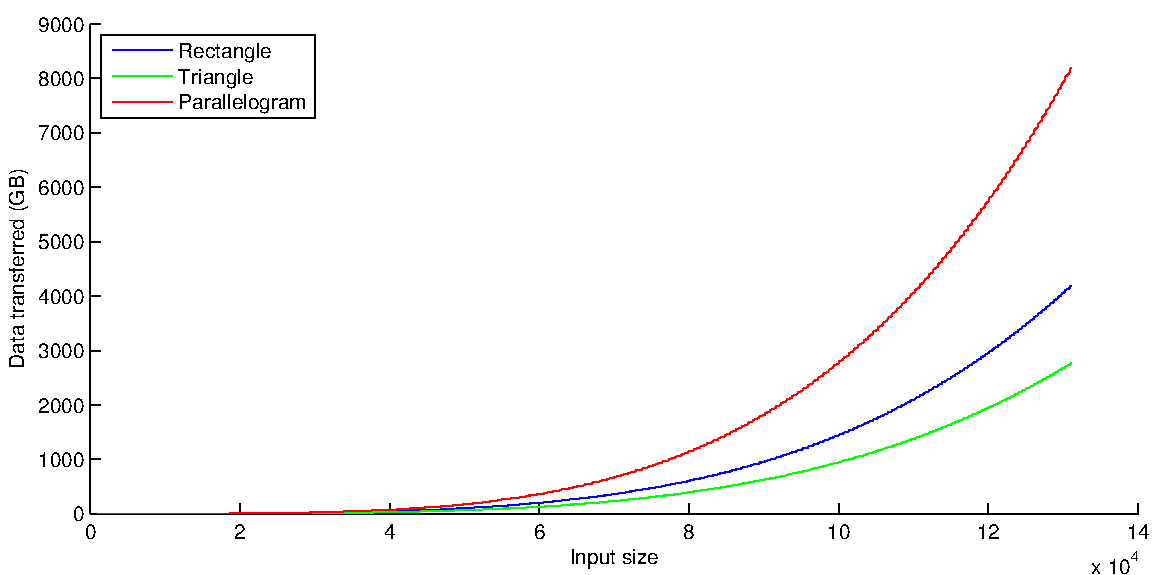
\includegraphics[width=14cm]{inc/ns_large.pdf}\end{center}

Given an experimental bandwidth of 5.3743 Gb/s between CPU and GPU, processing matrices one order of magnitude larger (128K) would result in respectively 13\up{(R)}, 8.5\up{(T)} and 25.4\up{(P)} minutes of transfer delay. Extrapolating the preliminary results of small problems, a computation on input of size 128K would require respectively 7 days 13h\up{(R)}, 2 days 22h\up{(T)} and 6 days 10h\up{(P)}, assuming there is no other scalability issues. Although this overhead seems appealing compared to the computation time, the total time blows up (because of the  $O(n^3)$ complexity) and make the processing of such large problem less relevant. Given that real problems -- like RNA folding -- operate at input sizes up to 4096, it would not be of much relevancy to implement a version for larger cases, although perfectly feasible.

% ----------------------------------------------
\subsubsection{Serial problems}
The serial problem have the interesting property to access to a fixed number of previous elements. These elements can be either stored either explicitly in a scoring matrix or implicitly as moving aggregation into a wavefront. Since the dependencies are fixed, the computation direction gains an additional degree of freedom: matrix can be solved in diagonal (as non-serial problems) or line-wise or column-wiser. This allows to store the whole necessary state to make progress into a limited number of lines (or columns), and sweep vertically (resp. horizontally) along the matrix.

Since serial problems are of complexity $O(n^2)$ (due to the matrix dimension and the finite number of dependencies), it is possible to tackle much larger problem than non-serial during the same running time. Hence, it seems obvious to let serial problems grow larger than the memory.

Mixing the dependency property and size requirements, we can split the matrix into sub-matrices, store special lines (and/or columns) into memory (or hard disk), and repeat computations to solve the backtrack (similarly as in \cite{swat_gpu},\cite{swat_mega}, but this implementation use problem-specific knowledge that might not generalize).

To store intermediate lines and columns, we are facing two different strategies to explore:\ul
\item \textbf{Fixed subproblem size:} we decompose the algorithm as follows\ol
\item Define a grid of <<major column and rows>>, where each cell's data (input, output, cost and backtrack matrices) fits into the device memory.
\item Compute the values of the grid's major columns and rows in one pass.
\item Second (on-demand) computation to process backtracking inside relevant cells.
\ole
Let $b$ the number of cells that we have on each row/column, the total computation running time would be $(b^2 + 2b) \cdot t_b$ where $t_b$ is the time to compute one cell's matrix. This division has the advantage of providing the minimal computation time at the expense of external storage proportional to $O(n)$ (if we store only lines or columns) or $O(n^2)$ (if we store both).

\item \textbf{Myers and Miller’s algorithm:} (divide and conquer)
This algorithm break the DP problem into 2 (or 4) subproblems such that once the middle line/column is computed, the problem can be solved for 1 submatrix and backtracking among up to 2 of the 3 other. This breaking is applied recursively until the submatrix data fits into memory. The storage requirements are $4 \cdot O(n)$ (we store along both dimension $1+\tfrac{1}{2}+\tfrac{1}{4}+...$ lines/columns).

The algorithm proceeds as follows: first it solves the problem to obtain the first backtracking element, then it breaks the matrix in 4 submatrices, and refine it until backtrack is tractable. Since there is at most $\log n/b$ refinements and since every part of the matrix may be involved in backtrack, running time is $O(n^2 \log_2 n)$.
\item \textbf{Hybrid approach:} a hybrid approach might be created to take advantage of additional available memory, however, the running time decreases logarithmically to the space used, this means that using twice more storage space would only result in a $2\times$ speedup (measuring only the computation time). Hence an hybrid approach would be to decide a $k$ such that at each step we partition the desired submatix into a intermediate grid of $k$ rows/columns. The space usage would be in $2 k \log_k (n/b)$ and the running time complexity would be $O(n^2 \cdot \log_k n)$. Then the user would be able to fix a storage space $S \ge 4 \log_2 (n/b)$ and obtain the corresponding $k$ for a given $n$.
\ule

{\color{red}
try to setup wavefront size (if needed) => just enlarge the matrix by 1 so that we go wavefront-to-wavefront

XXX: what's the maximal size of the wavefront ??

XXX: can we avoid to store some matrices and put them in the wavefront ??

Split into blocks:\ul
\item Decide the shape of the blocks
\item Decide the size of the blocks
\item Decide of a strategy to store intermediate lines/columns: space/time tradeoff.
\ule

XXX: make it work up to 14K for all 3 problems using multiple kernels
XXX: example of non-symmetric serial problem

The three last elements, combined with the above one, provide a precise estimation of the memory consumption, and the implementation difficulty 

all the problem are subject to the input dimensions $n$.

the two latter one gives an estimation of the constant factor.

The delay of dependencies might also have an impact: if the matrix is too large to fit in the memory (device or main memory), it becomes necessary to maintain partial matrix content (all the intermediate elements) within the wavefront. Also the number of cost matrices might affect the performance, simply because maintaining them requires computations and memory accesses.
}

% ------------------------------------------------------------------------------------------------
\subsection{Memory layout}
{\color{red} XXX}


% ------------------------------------------------------------------------------------------------
\newpage
{\color{red} 
\subsection{LMS compiler stack}
\textbf{User-language}: define additional parameters for the recurrence\ul
\item Windowing (to convert non-serial into serial problems)
\item Input sizes, and alphabets (backtrack, input, cost)
\item Backtrack (implicitly by backtrack alphabet size) and cost matrices bit-sizes (cost maximum may be inferred using <<Yield size/grammar analysis>>)
\item Recurrence functions, devices available
\item What to keep in memory (cost, backtrack or both).
\ule
$\Downarrow$ Conversion (using an existing technique)

\textbf{Intermediate representation}

$\Downarrow$ Optimizations\ul
\item Transform non-serial into serial \ul
	\item Use aggregation functions/transformations
	\item Use windowing from user (if no other technique succeed)
	\ule
\item Define the wavefront depth
\item Avoiding the cost matrix by moving it into the wavefront
\ule

\textbf{Code specification}\ul
\item Kernel function (1-element function), inputs, outputs, wave front, dependencies, bit sizes
\item Device-level interface => setup the block sizes(w/h), input and memory sizes
\item Define the device-specific implementation of the block (CPU/FPGA/CUDA)
\item Define the co-processor memory aggregation function
\item Define the scheduling of the blocks and aggregation (software pipelining)
\item Define the data movement back and forth to disk
\ule

$\Downarrow$ Generation\ul
\item Generate the kernel for specific device
\item Generate the scheduling and barriers
\ule

\textbf{Binary program}
}
%\ol
%\item Make sure we encompass all the most common patterns of DP: check if we have higher dimensions or more complex formula.
%\item Let the user tune the window size if he wants to reduce non-serial to serial.
%\item Concerns separation: common architecture enables flexibility (exchange components) \ul
%	\item Block processor: CPU, GPU, FPGA, must allow variation of width and height
%	\item Memory stats computation (min, sum, ... column/line combinations): CPU, GPU
%	\item Scheduler (CPU): interleave block computation and memory statistics
%	\ule
%\item Common description \ul
%	\item Block kernel processor
%	\item Full block
%	\ule
%\item Discussion: wavefront, design similarities, polyhedral theory
%\ole

%%\newcolumntype{C}[1]{>{\centering\let\newline\\\arraybackslash}m{#1}}
%\newcolumntype{C}{@{\hspace{7pt}}c@{\hspace{7pt}}}
%\def\mnl{\rule{0pt}{2.6ex}\rule[-1.2ex]{0pt}{0pt} \\ \hline}
%$\begin{array}{|C|C|C|C|C|C|} \hline
%0 & 0 & 0 & 0 & 0 & 0 \mnl
%0 &  &  &  &  & \mnl
%0 & M_{23}  &  &  &  & \mnl
%0 &  & \sum  &  &  & \mnl
%0 &  &  &  &  & \mnl
%0 &  &  &  &  & \mnl
%\end{array}$
%\end{document}
